

\subsubsection{s$^3$hark}
The panel for this event application is as shown in \autoref{fig:s3hark0}. 
This application does effective free-field site response analysis of a soil column.
In this panel the user specifies a ground motion at the bottom of the column. 
With soil layer properly defined, the motion at the ground surface will be given at the end of the analysis.
\begin{figure}[!htbp]
  \centering {
    
\includegraphics[width=0.8\textwidth]
    {figs/s3hark0.png} }
  \caption{s$^3$hark}
  \label{fig:s3hark0}
\end{figure}

The UI of s$^3$hark is shown in \autoref{fig:s3hark1}.
There are two graphics shown in the left of the panel. The first one is the soil column graphic, 
which shows a visualization of the soil column.
The second one is the mesh and profile graphic, 
which shows the finite element mesh and profile plots.
On the right of the panel are operation area, soil design table, configure tab, layer property tab and response tab. 


\begin{figure}[!htbp]
  \centering {
    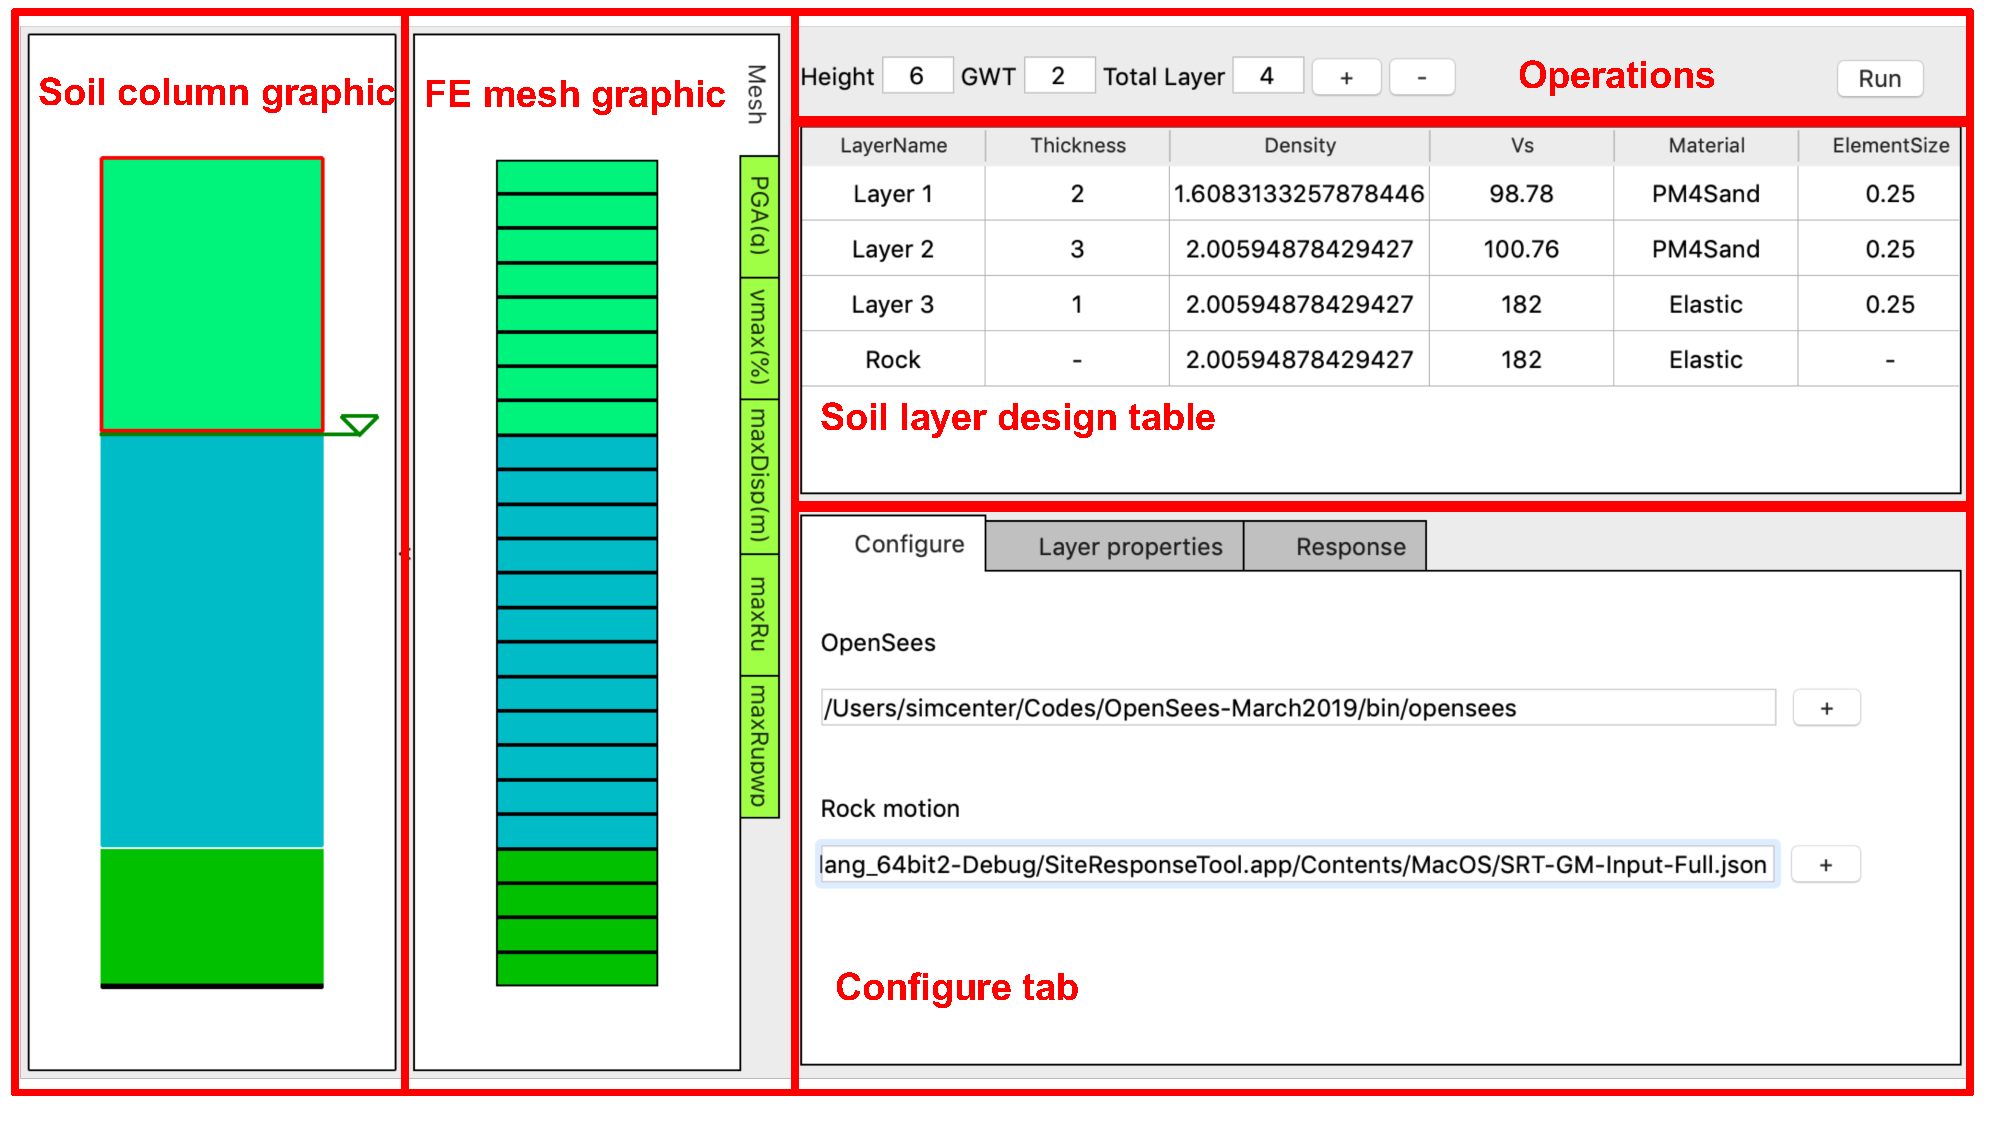
\includegraphics[width=0.8\textwidth]
    {figs/s3hark1.pdf} }
  \caption{s$^3$hark - Panels}
  \label{fig:s3hark1}
\end{figure}

In the operation area as shown in \autoref{fig:s3hark2}, click the plus button to add a layer and the minors button to delete a selected layer. 
Change the ground water table in the GWT input field. 
In the configure tab, path of OpenSees executable and rock motion file need to be specified.
A click on the run button will start the finite element analysis.


\begin{figure}[!htbp]
  \centering {
    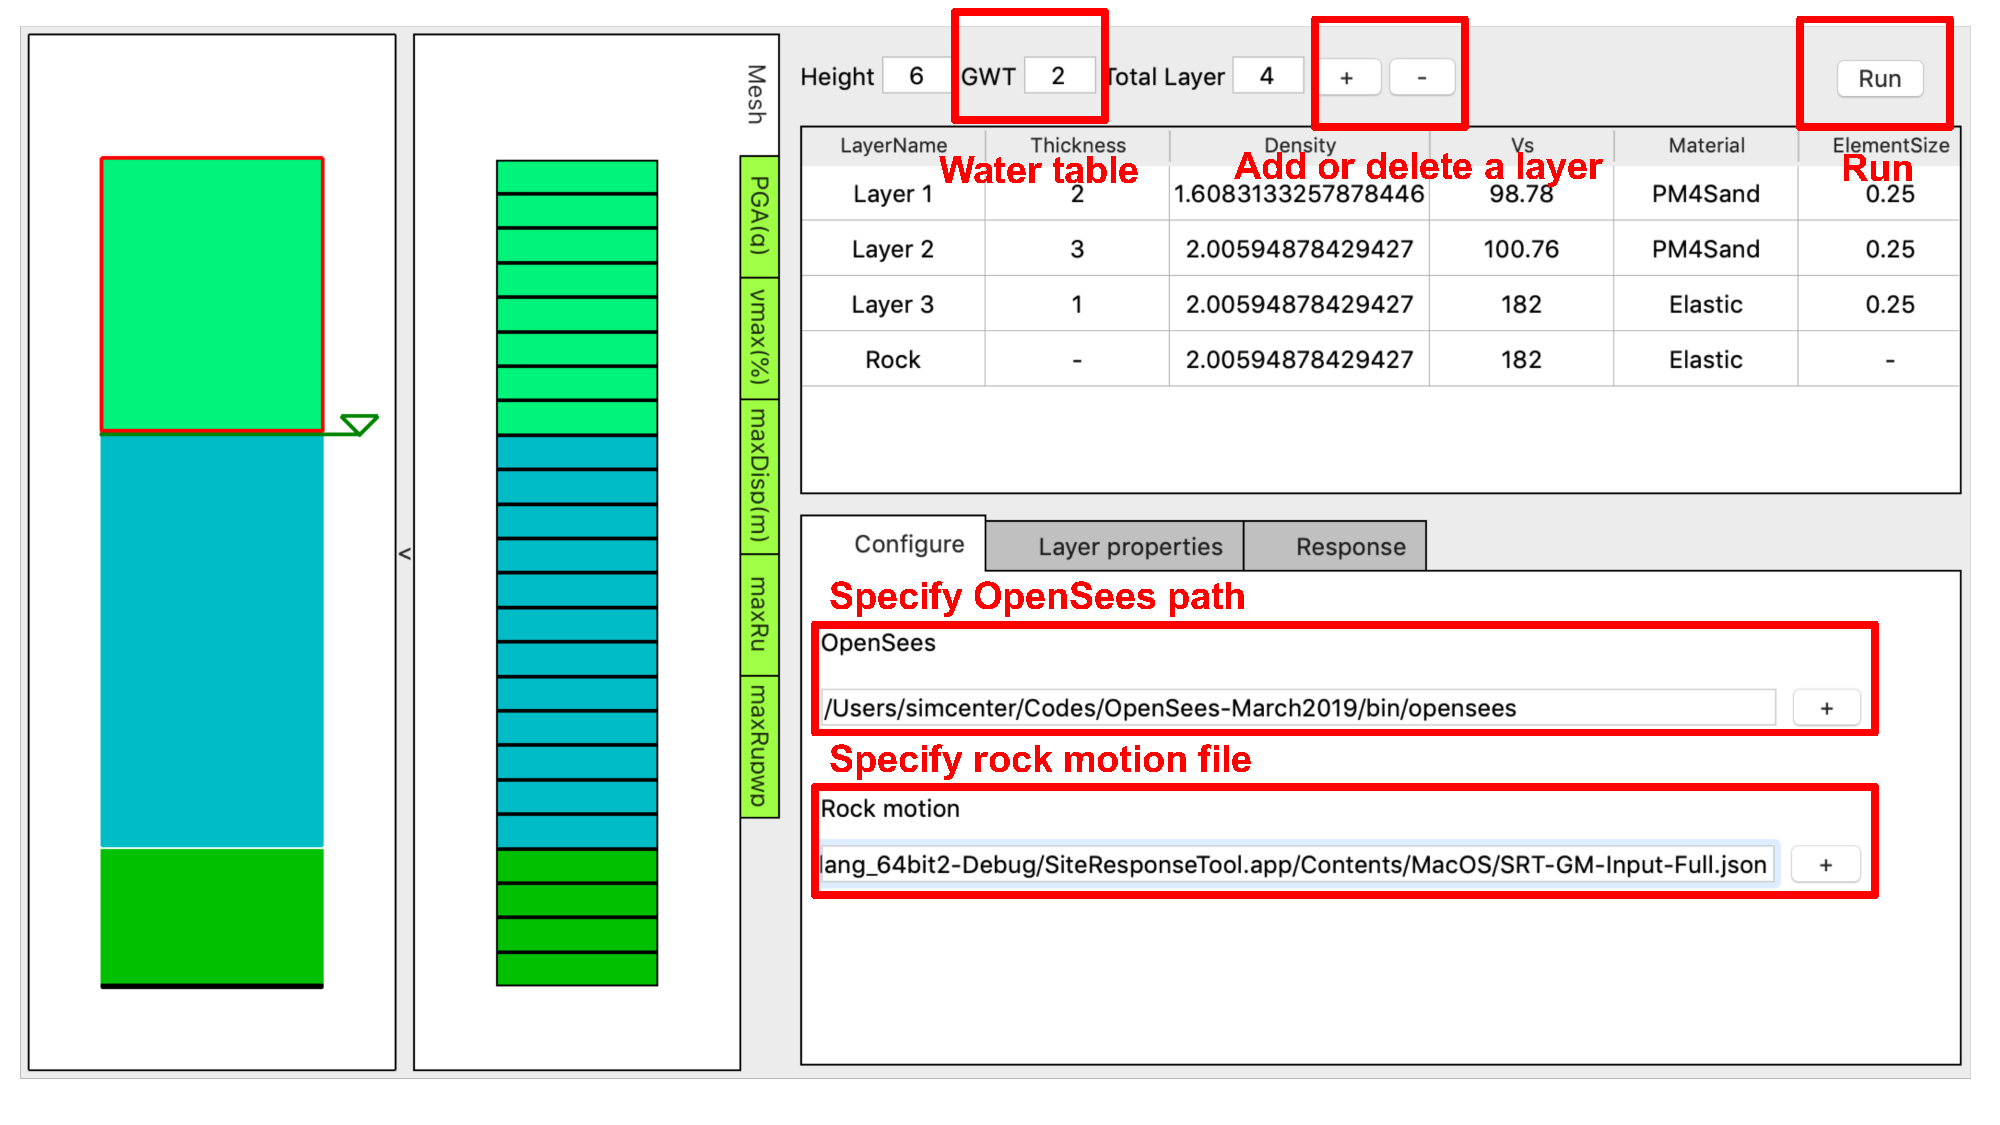
\includegraphics[width=0.8\textwidth]
    {figs/s3hark2.pdf} }
  \caption{s$^3$hark - Configurations and Operations }
  \label{fig:s3hark2}
\end{figure}

Either click on the soil column or the table to select a layer \autoref{fig:s3hark3}. 
When a layer is selected, it will be highlighted in both the soil column graphic and the table. 
Selection of a soil layer will invoke the Layer properties tab, where the user can specify the material properties of this layer.
Double click on a cell of the table will allow the user to change the corresponding value.

\begin{figure}[!htbp]
  \centering {
    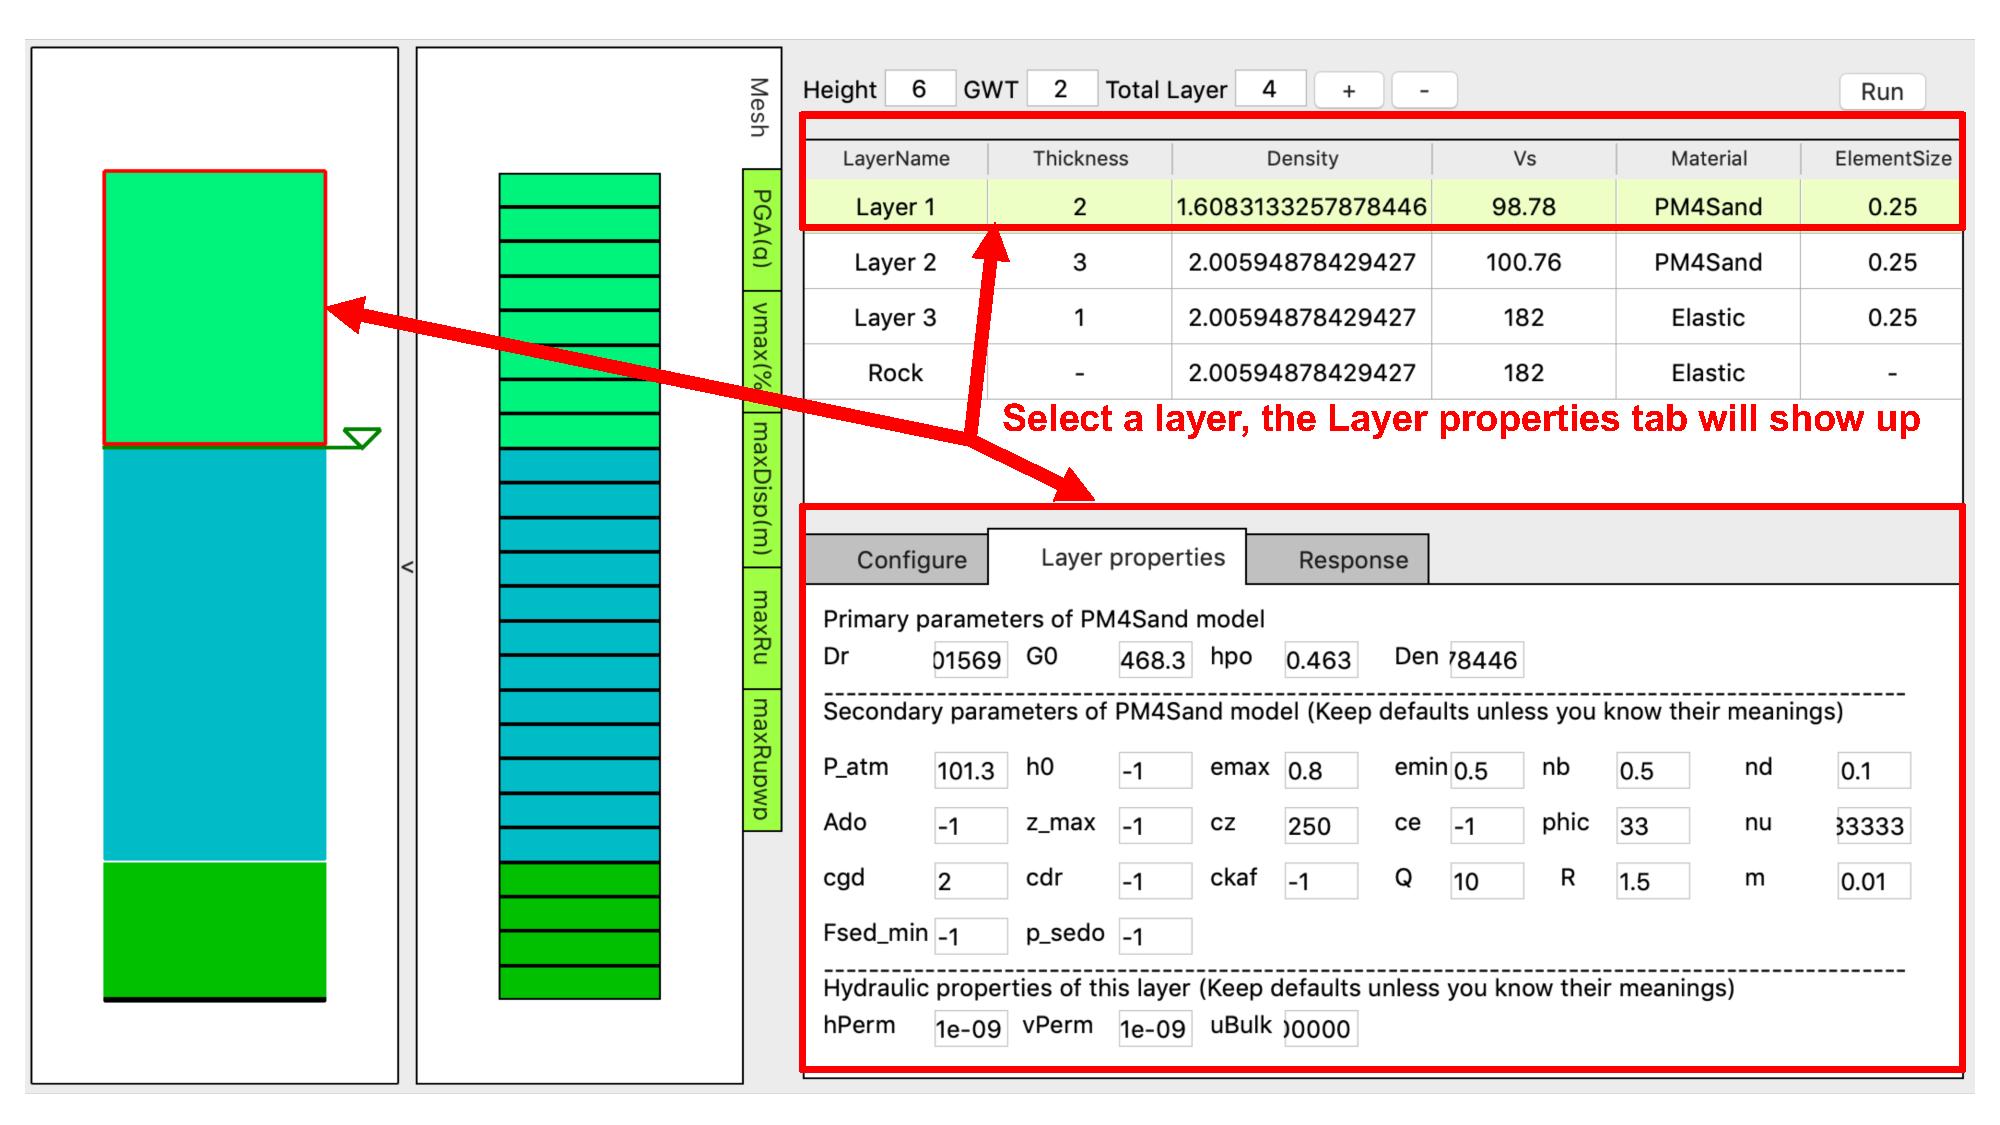
\includegraphics[width=0.8\textwidth]
    {figs/s3hark3.pdf} }
  \caption{s$^3$hark - Layer modification }
  \label{fig:s3hark3}
\end{figure}


Upon the finish of the finite element analysis, the ground motion at the soil surface (\autoref{fig:s3hark4}) will be stored in EE-UQ's input file.
This computed motion will be later applied to the bottom of the building.

\begin{figure}[!htbp]
  \centering {
    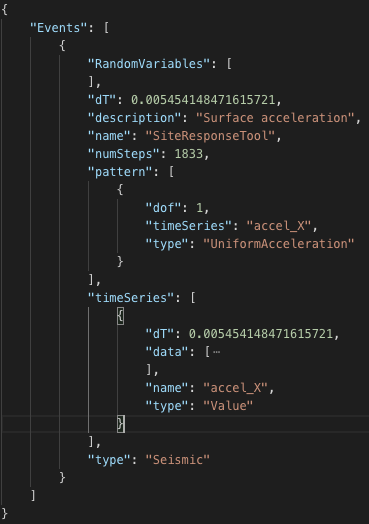
\includegraphics[width=0.4\textwidth]
    {figs/s3hark4.png} }
  \caption{s$^3$hark - Surface motion }
  \label{fig:s3hark4}
\end{figure}




\subsubsection{s$^3$hark verification}

A 2D free field effective stress analysis is performed by s$^3$hark and demonstrated here. 
The results are verified against FLAC and Plaxis. 
The soil column being analyzed is 6 meters high sitting on a rock.
The ground water table is at 2 meters below the soil surface.
In the column, there are a total of three soil layers. Each layer is meshed by elements with a size of 0.25 meter in height.
Basic properties of soil layers and the rock are shown in \autoref{fig:s3harkSoilColumn} and \autoref{fig:s3hark5}.
The first two layers are modeled by PM4Sand and the third layer is modeled by elastic isotropic material. 
(The implementation work of PM4Sand \cite{boulanger2015pm4sand} is done in University of Washington by Long Chen and Pedro Arduino.
Chaofeng Wang at UC, Berkeley contributed to the code optimization for speed improvement. )
The rock layer will be simplified to a \cite{Lysmer:1969}  dashpot, which accounts for the finite rigidity of the underlying elastic medium.
The parameters of the dashpot are calculated solely based on rock layer's density and V$_{s30}$.


\begin{figure}[!htbp]
  \centering {
    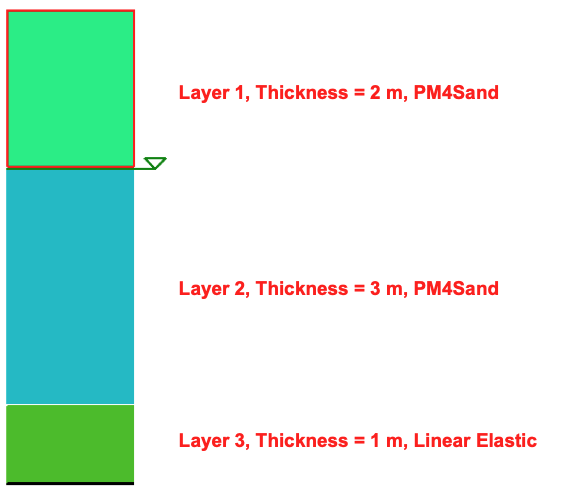
\includegraphics[width=0.5\textwidth]
    {figs/s3harkSoilColumn.png} }
  \caption{Soil layers }
  \label{fig:s3harkSoilColumn}
\end{figure}


\begin{figure}[!htbp]
  \centering {
    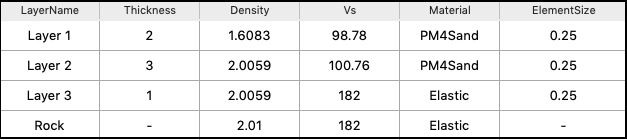
\includegraphics[width=0.5\textwidth]
    {figs/s3hark5.png} }
  \caption{Soil layers }
  \label{fig:s3hark5}
\end{figure}


The detailed properties of the material in each soil layer are shown in \autoref{fig:s3hark6}.

\begin{figure}[!htbp]
  \centering 
  \subfloat[Layer 1]{
    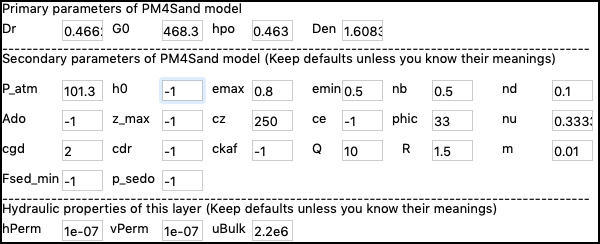
\includegraphics[width=0.4\textwidth]
    {figs/layer1.png}}
  \subfloat[Layer 2]{
    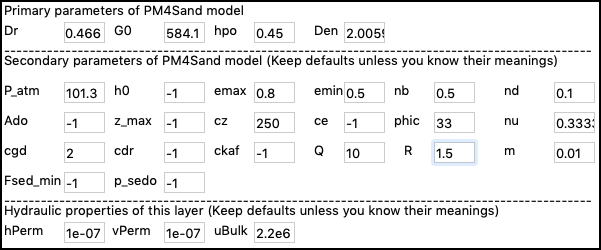
\includegraphics[width=0.39\textwidth]
    {figs/layer2.png}}
    
    \subfloat[Layer 3]{
    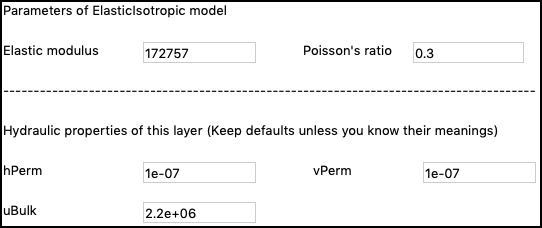
\includegraphics[width=0.4\textwidth]
    {figs/layer3.png}}
  \caption{Detail soil properties and material model parameters}
  \label{fig:s3hark6}
\end{figure}

For the verification and validation purposes, s$^3$hark's results are compared with FLAC an PLAXIS, as shown in \autoref{fig:s3hark7}. 
All three programs generally produce very similar response with
different levels of differences shown in PHA, maximum shear strain, CSR, maximum pore pressure ratio. 
The differences come from multiple sources, such as numerical discretization methods, solvers, etc.
For example, FLAC tends to produce higher dilation pulses in liquefied layer. 
This is possibly due to a combination of different reasons, e.g.,
interpolation of data from integration points at different
locations, numerical methods for integration, formulations for
solid fluid coupling, etc.
(Chaofeng Wang at UC, Berkeley, Long Chen and Andrew Makdisi at University of Washington,  
Gregor Vilhar at PLAXIS, BV contributed to the verification of PM4Sand in s$^3$hark. )

\begin{figure}[!htbp]
  \centering {
    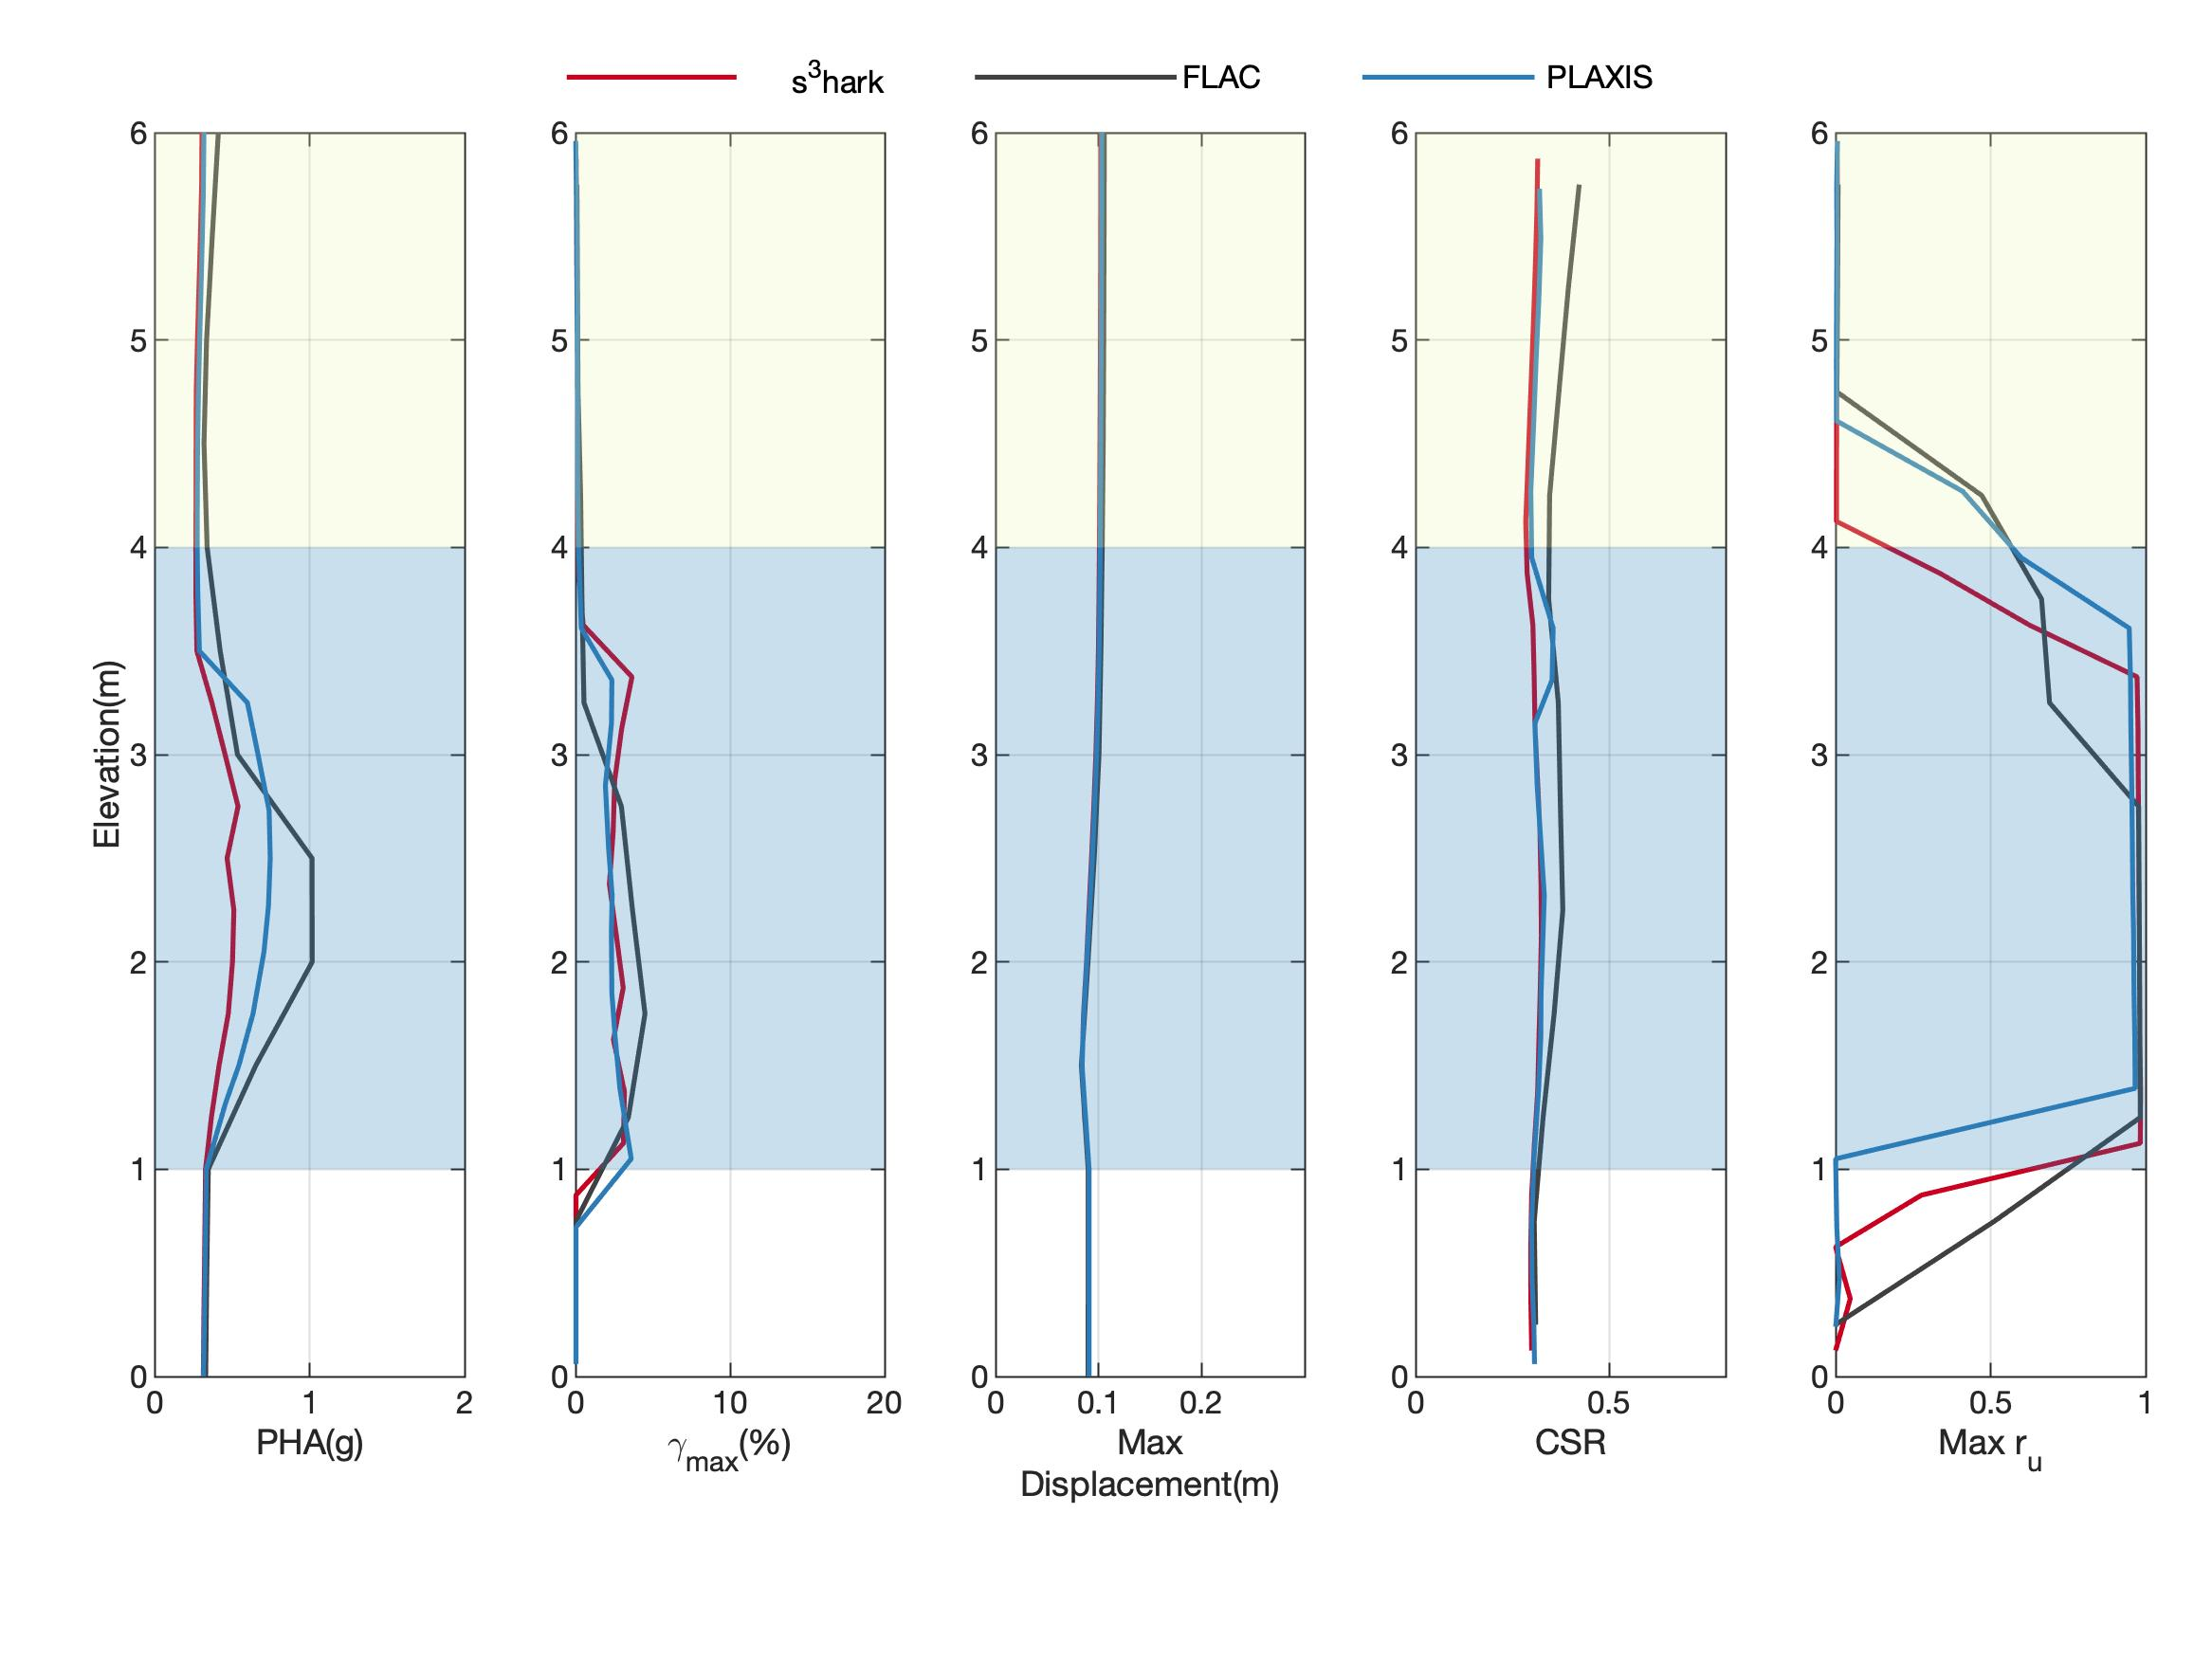
\includegraphics[width=0.7\textwidth]
    {figs/N10T3_RSN766_ProfileCompare.jpg} }
  \caption{Soil layers }
  \label{fig:s3hark7}
\end{figure}





